% Numerical reference: asset/BRL_EXP/05; originals retained in 05_exp_system.tex.
\subsection{System Evaluation}~\label{exp:sys_eval}
\begin{table}[t]
\centering
\captionsetup{font=small,skip=5pt}
\caption{Query \textbf{timing} (when) and query \textbf{selection} (what) strategies. KnowNo, IntroPlan and POMCP-Q are the baselines. R, S1--S2 and T1--T3 are the ablation configurations. A dash denotes a combination not evaluated in this study.}
\label{tab:query_strategy_matrix}
\footnotesize
\setlength{\tabcolsep}{1pt}
\renewcommand{\arraystretch}{1.15}
\arrayrulecolor{black}
\begin{tabular*}{\columnwidth}{@{\extracolsep{\fill}}lcccc@{}}
\toprule
\diagbox[innerwidth=\widthof{Conformal Set},height=0.85cm,dir=NW,linewidth=0.3pt,font=\bfseries]{What}{When} & Random & \makecell[c]{Conformal\\Prediction} & \makecell[c]{Reward-\\based} & Confidence \\
\midrule
Random & R & -- & -- & S1 \\
\addlinespace[3pt]
Conformal Set & -- & \makecell[c]{KnowNo,\\IntroPlan} & -- & -- \\
\addlinespace[3pt]
Reward-based & -- & -- & POMCP-Q & S2 \\
\addlinespace[3pt]
Entropy Gain & T1 & T2 & T3 & \textbf{Ours} \\
\bottomrule
\end{tabular*}
\end{table}

Table~\ref{tab:query_strategy_matrix} summarizes the baseline and ablation configurations. The baseline comparison in Sec.~\ref{exp:sys_baseline} evaluates KnowNo, IntroPlan, and POMCP-Q against Ours. This comparison evaluates complete task planning systems that query an external agent to plan and execute actions. We evaluate these systems with oracle, VLM, and human feedback to examine whether the observed performance trends persist across feedback sources. The ablation study in Sec.~\ref{exp:policy_ablation} evaluates R, S1--S2, and T1--T3 against Ours where T1--T3 examine query timing (when) and S1--S2 examine query selection (what). Finally the threshold study in Sec.~\ref{exp:sys_threshold} examines how the confidence threshold affects task success and query count. Both the ablation and threshold studies use oracle responses in simulation.



\subsubsection{Baseline Comparison}~\label{exp:sys_baseline}
\noindent\textbf{Oracle}. The oracle comparison includes three baselines with the query timing and selection strategies summarized in Table~\ref{tab:query_strategy_matrix}. KnowNo~\citep{ren2023robots} requests an action choice if its conformal prediction set does not specify a single ordinary action. IntroPlan~\citep{liang2024introspective} extends KnowNo and incorporates retrieved examples and explanations into candidate evaluation before it requests an action choice. We implement a HARPS-inspired POMCP baseline (POMCP-Q)~\citep{burks2023harps} that selects between physical actions and Boolean queries to an external agent by maximizing expected cumulative reward. We adapt HARPS to our symbolic task domains, executing physical actions and queries separately. Table~\ref{tab:baseline_results} and Fig.~\ref{fig:baseline_results} compare the four methods.

\begin{figure*}[!tp]
\centering
\begin{subfigure}[t]{0.247\textwidth}
\centering
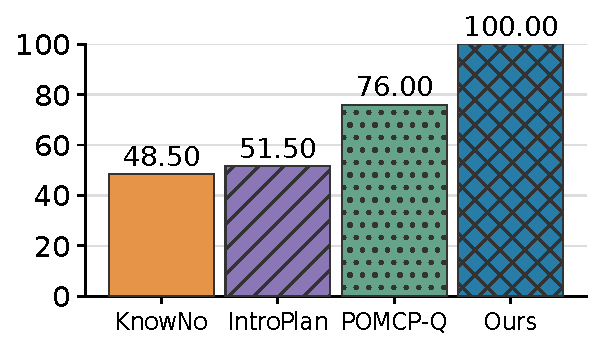
\includegraphics[width=\linewidth,height=.16\textheight,keepaspectratio]{figures/04_ORACLE_BASELINE/exp_oracle_waste_success.pdf}
\caption{Sort Success rate (\%)}
\label{fig:baseline_oracle_waste_success}
\end{subfigure}%
\hspace{0.004\textwidth}%
\begin{subfigure}[t]{0.247\textwidth}
\centering
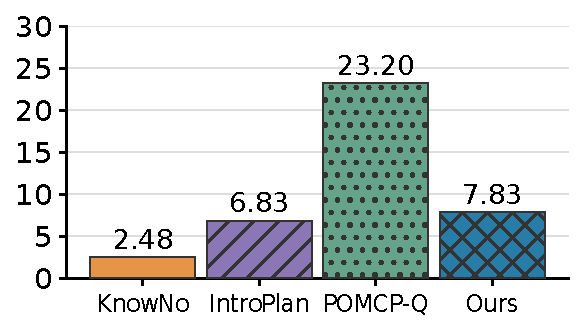
\includegraphics[width=\linewidth,height=.16\textheight,keepaspectratio]{figures/04_ORACLE_BASELINE/exp_oracle_waste_queries.pdf}
\caption{Sort Query count}
\label{fig:baseline_oracle_waste_queries}
\end{subfigure}%
\hspace{0.004\textwidth}%
\begin{subfigure}[t]{0.247\textwidth}
\centering
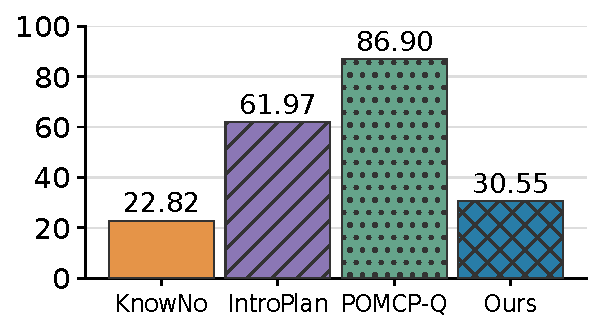
\includegraphics[width=\linewidth,height=.16\textheight,keepaspectratio]{figures/04_ORACLE_BASELINE/exp_oracle_waste_query_probability.pdf}
\caption{Sort Query prob. (\%)}
\label{fig:baseline_oracle_waste_query_probability}
\end{subfigure}%
\hspace{0.004\textwidth}%
\begin{subfigure}[t]{0.247\textwidth}
\centering
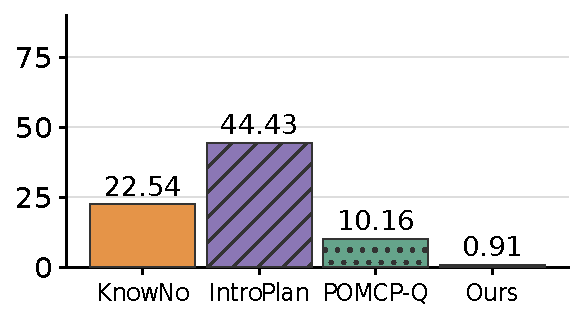
\includegraphics[width=\linewidth,height=.16\textheight,keepaspectratio]{figures/04_ORACLE_BASELINE/exp_oracle_waste_plan_time.pdf}
\caption{Sort Plan time (s)}
\label{fig:baseline_oracle_waste_plan_time}
\end{subfigure}
\par\smallskip
\begin{subfigure}[t]{0.247\textwidth}
\centering
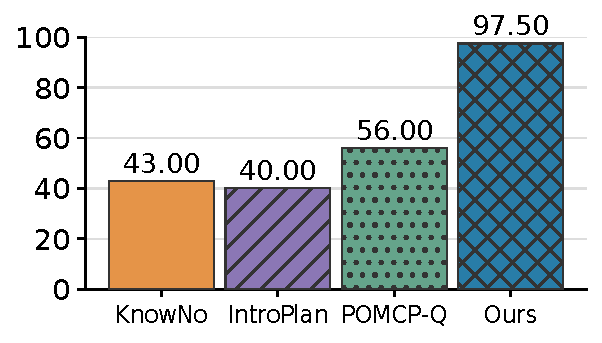
\includegraphics[width=\linewidth,height=.16\textheight,keepaspectratio]{figures/04_ORACLE_BASELINE/exp_oracle_tomato_success.pdf}
\caption{Harvest Success rate (\%)}
\label{fig:baseline_oracle_tomato_success}
\end{subfigure}%
\hspace{0.004\textwidth}%
\begin{subfigure}[t]{0.247\textwidth}
\centering
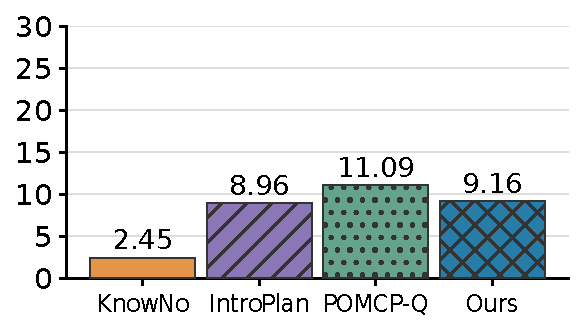
\includegraphics[width=\linewidth,height=.16\textheight,keepaspectratio]{figures/04_ORACLE_BASELINE/exp_oracle_tomato_queries.pdf}
\caption{Harvest Query count}
\label{fig:baseline_oracle_tomato_queries}
\end{subfigure}%
\hspace{0.004\textwidth}%
\begin{subfigure}[t]{0.247\textwidth}
\centering
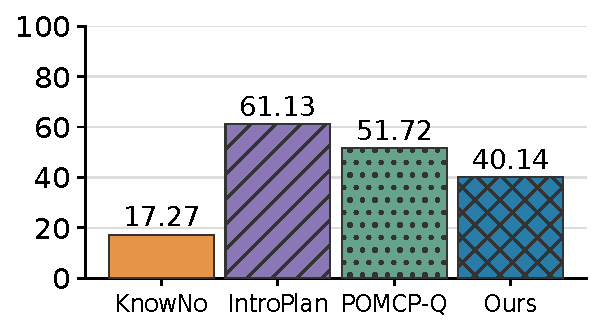
\includegraphics[width=\linewidth,height=.16\textheight,keepaspectratio]{figures/04_ORACLE_BASELINE/exp_oracle_tomato_query_probability.pdf}
\caption{Harvest Query prob. (\%)}
\label{fig:baseline_oracle_tomato_query_probability}
\end{subfigure}%
\hspace{0.004\textwidth}%
\begin{subfigure}[t]{0.247\textwidth}
\centering
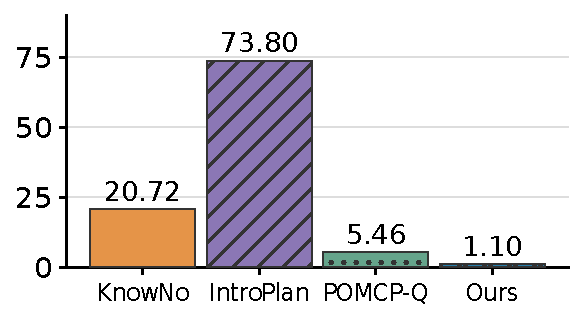
\includegraphics[width=\linewidth,height=.16\textheight,keepaspectratio]{figures/04_ORACLE_BASELINE/exp_oracle_tomato_plan_time.pdf}
\caption{Harvest Plan time (s)}
\label{fig:baseline_oracle_tomato_plan_time}
\end{subfigure}
\caption{Oracle baseline comparison. (a), (e) Ours achieves the highest success rates in both domains. (b)-(c), (f)-(g) Ours uses more queries than KnowNo and IntroPlan but fewer than POMCP-Q, with a lower query probability than IntroPlan and POMCP-Q. (d), (h) Ours has the shortest plan times in both domains. These results indicate that query count alone does not explain task success or plan time.}
\label{fig:baseline_results}
\end{figure*}





% As shown in Table~\ref{tab:baseline_results} and Fig.~\ref{fig:baseline_results}, our method achieves the highest success rate in both domains. It completes all $200$ Sort trials and $196$ of $200$ Harvest trials. Our method achieves success rates of $100.00\%$ in Sort and $98.00\%$ in Harvest compared with $87.00\%$ and $57.50\%$ for POMCP-Q. The mean query counts are also lower at $7.83$ and $9.16$ compared with $24.52$ and $11.28$ for POMCP-Q. Two factors may explain the lower success rate and higher query count of POMCP-Q. First, query actions expand the action space so POMCP must evaluate more alternatives within the same simulation budget. Second, expected task reward does not explicitly measure confidence in the current state. Our method selects queries at the observation stage and restricts POMCP planning to physical actions. These results show that a higher query count alone does not guarantee a higher success rate.

% Compared to KnowNo and IntroPlan, our method uses more queries. Their mean query counts are $2.48$ and $6.83$ in Sort compared with $7.83$ for our method. In Harvest, the corresponding counts are $2.45$ and $8.96$ compared with $9.16$ for our method. This difference in query count arises from how each method handles a query trigger. If a query is triggered, our method repeats queries until belief confidence reaches $\tau$. KnowNo and IntroPlan ask only one question per trigger. Therefore our method can use more queries despite a lower query probability than IntroPlan. However KnowNo and IntroPlan achieve success rates of only $48.50\%$ and $51.50\%$ in Sort and $43.00\%$ and $40.00\%$ in Harvest. Therefore a system is not necessarily better simply because it uses fewer queries.

% Plan time is also lowest for Ours in both domains despite the additional queries compared with KnowNo and IntroPlan. In Sort, mean plan time is $0.91$ seconds for Ours compared with $22.54$ seconds for KnowNo, $44.43$ seconds for IntroPlan, and $10.47$ seconds for POMCP-Q. In Harvest, the corresponding values are $1.10$, $20.72$, $73.80$, and $5.55$ seconds. KnowNo and IntroPlan require language-model inference for candidate generation and scoring at each planning step. IntroPlan performs additional reasoning and candidate evaluation, which increases inference time compared with KnowNo. Ours evaluates query timing and selection from the belief state and searches only over physical actions. The smaller search space supports faster planning than POMCP-Q. The time comparisons suggest that belief-based search can reduce plan time without repeated language-model inference. % Therefore a higher query count does not necessarily imply a higher planning cost.

% Our method combines confidence-based query timing with entropy gain query selection and achieves the highest success rate in both domains. The baseline comparisons suggest that effective query timing and selection are more important than query count alone.

As shown in Table~\ref{tab:baseline_results} and Fig.~\ref{fig:baseline_results}, Ours achieves success rates of $100.00\%$ in Sort and $97.50\%$ in Harvest, compared with $76.00\%$ and $56.00\%$ for POMCP-Q, while using fewer queries in both domains. POMCP-Q includes queries in the action space, increasing the alternatives evaluated within a fixed simulation budget. Its reward criterion also does not explicitly assess confidence in the current state. These differences may contribute to its lower success rate and higher query count. Ours verifies state facts after observations and restricts action planning to physical actions.

Ours uses more queries than KnowNo and IntroPlan because it continues verification until belief confidence reaches $\tau$, whereas both baselines request one action choice per trigger. This distinction explains how Ours can have a lower query probability than IntroPlan while asking more questions overall. Similar query counts also yield substantially different outcomes. In Harvest, IntroPlan and Ours use $8.96$ and $9.16$ queries, respectively, yet achieve success rates of $40.00\%$ and $97.50\%$. Query count alone therefore does not explain task success.

Ours also has the lowest plan time in both domains. KnowNo and IntroPlan invoke a language model for candidate generation and scoring, with IntroPlan additionally generating explanations for candidate evaluation. Ours computes query timing and selection from the belief state and searches over physical actions only. This avoids repeated language-model inference and limits the search space compared with POMCP-Q.



\begin{table*}[t]
\centering
\caption{Baseline results. Underlines mark best means.}
\label{tab:baseline_results}
\footnotesize
\setlength{\tabcolsep}{2pt}
\renewcommand{\arraystretch}{1.05}
\setlength{\extrarowheight}{0pt}
\medmuskip=1mu\relax
\begin{tabular*}{\textwidth}{@{\extracolsep{\fill}}llccccccc@{}}
% \begin{tabular}{llcccc}
\toprule
Setting & Method & Success (\%) & Query count & Query prob.(\%) & Plan length & Total time (s) & Inter. time (s) & Plan time (s)\\
\midrule
\multirow{4}{*}{\shortstack[l]{Oracle\\Sort}} & KnowNo & 48.50 & $\underline{2.48} \pm 1.42$ & $\underline{22.82} \pm 12.61$ & $10.78 \pm 1.35$ & $22.54 \pm 3.04$ & - & $22.54 \pm 3.04$ \\
 & IntroPlan & 51.50 & $6.83 \pm 1.53$ & $61.97 \pm 9.35$ & $10.99 \pm 1.49$ & $44.43 \pm 8.05$ & - & $44.43 \pm 8.05$ \\
 & POMCP-Q & 76.00 & $23.20 \pm 4.39$ & $86.90 \pm 5.29$ & $11.72 \pm 1.49$ & $10.16 \pm 1.36$ & - & $10.16 \pm 1.36$ \\
 & \textbf{Ours} & \textbf{\underline{100.00}} & $\boldsymbol{7.83 \pm 2.16}$ & $\boldsymbol{30.55 \pm 10.41}$ & $\boldsymbol{\underline{10.35} \pm 0.88}$ & $\boldsymbol{\underline{0.91} \pm 0.09}$ & - & $\boldsymbol{\underline{0.91} \pm 0.09}$ \\
\addlinespace[3pt]
\multirow{4}{*}{\shortstack[l]{Oracle\\Harvest}} & KnowNo & 43.00 & $\underline{2.45} \pm 1.06$ & $\underline{17.27} \pm 6.67$ & $14.01 \pm 1.07$ & $20.72 \pm 2.25$ & - & $20.72 \pm 2.25$ \\
 & IntroPlan & 40.00 & $8.96 \pm 2.04$ & $61.13 \pm 10.77$ & $14.61 \pm 1.46$ & $73.80 \pm 8.96$ & - & $73.80 \pm 8.96$ \\
 & POMCP-Q & 56.00 & $11.09 \pm 3.59$ & $51.72 \pm 10.50$ & $14.77 \pm 1.36$ & $5.46 \pm 1.11$ & - & $5.46 \pm 1.11$ \\
 & \textbf{Ours} & \textbf{\underline{97.50}} & $\boldsymbol{9.16 \pm 1.91}$ & $\boldsymbol{40.14 \pm 4.50}$ & $\boldsymbol{\underline{13.93} \pm 1.03}$ & $\boldsymbol{\underline{1.10} \pm 0.16}$ & - & $\boldsymbol{\underline{1.10} \pm 0.16}$ \\
\specialrule{0.4pt}{\aboverulesep}{1pt}\specialrule{0.4pt}{0pt}{\belowrulesep}
\multirow{2}{*}{\shortstack[l]{VLM\\Sort}} & KnowNo & 50.00 & $\underline{3.15} \pm 0.88$ & $28.64 \pm 7.96$ & $\underline{11.00} \pm 0.00$ & $\underline{186.51} \pm 10.90$ & $\underline{15.46} \pm 4.45$ & $19.99 \pm 4.76$ \\
 & \textbf{Ours} & \textbf{\underline{92.50}} & $\boldsymbol{6.70 \pm 1.76}$ & $\boldsymbol{\underline{19.81} \pm 3.27}$ & $\boldsymbol{11.24 \pm 0.49}$ & $\boldsymbol{193.69 \pm 13.52}$ & $\boldsymbol{26.83 \pm 7.76}$ & $\boldsymbol{\underline{0.99} \pm 0.05}$ \\
\addlinespace[3pt]
\multirow{2}{*}{\shortstack[l]{VLM\\Harvest}} & KnowNo & 25.00 & $\underline{7.20} \pm 1.87$ & $44.10 \pm 7.51$ & $16.10 \pm 1.73$ & $217.82 \pm 17.78$ & $44.99 \pm 13.10$ & $26.90 \pm 3.07$ \\
 & \textbf{Ours} & \textbf{\underline{92.50}} & $\boldsymbol{8.51 \pm 1.52}$ & $\boldsymbol{\underline{37.63} \pm 3.04}$ & $\boldsymbol{\underline{13.27} \pm 0.77}$ & $\boldsymbol{\underline{180.39} \pm 11.18}$ & $\boldsymbol{\underline{34.12} \pm 7.62}$ & $\boldsymbol{\underline{1.38} \pm 0.19}$ \\
\specialrule{0.4pt}{\aboverulesep}{1pt}\specialrule{0.4pt}{0pt}{\belowrulesep}
\multirow{2}{*}{\shortstack[l]{Human\\Sort}} & KnowNo & 20.00 & $\underline{3.00} \pm 1.41$ & $25.76 \pm 10.71$ & $11.50 \pm 0.71$ & $\underline{184.48} \pm 24.08$ & $\underline{11.59} \pm 7.94$ & $16.94 \pm 0.39$ \\
 & \textbf{Ours} & \textbf{\underline{90.00}} & $\boldsymbol{7.11 \pm 1.83}$ & $\boldsymbol{\underline{18.18} \pm 0.00}$ & $\boldsymbol{\underline{11.00} \pm 0.00}$ & $\boldsymbol{190.15 \pm 50.72}$ & $\boldsymbol{36.49 \pm 47.55}$ & $\boldsymbol{\underline{0.94} \pm 0.04}$ \\
\addlinespace[3pt]
\multirow{2}{*}{\shortstack[l]{Human\\Harvest}} & KnowNo & 30.00 & $\underline{3.67} \pm 0.58$ & $\underline{28.21} \pm 4.44$ & $\underline{13.00} \pm 0.00$ & $195.50 \pm 8.26$ & $\underline{19.04} \pm 8.16$ & $23.52 \pm 1.21$ \\
 & \textbf{Ours} & \textbf{\underline{100.00}} & $\boldsymbol{8.50 \pm 1.78}$ & $\boldsymbol{37.36 \pm 3.74}$ & $\boldsymbol{13.10 \pm 0.32}$ & $\boldsymbol{\underline{180.02} \pm 13.14}$ & $\boldsymbol{23.89 \pm 13.47}$ & $\boldsymbol{\underline{1.32} \pm 0.08}$ \\
\bottomrule
\end{tabular*}
\end{table*}












\vspace{10pt}
\noindent\textbf{VLM}\label{exp:vlm_eval}.
We evaluate whether the oracle trends persist with VLM feedback on physical robots.\footnote{Appendix~\ref{appx:vlm_prompts} provides the VLM prompts.} We select KnowNo because it achieves success rates similar to IntroPlan with fewer queries than either IntroPlan or POMCP-Q in the oracle experiments. The physical experiments compare task success and interaction costs between Ours and KnowNo. We conduct $40$ trials per method and domain. Fig.~\ref{fig:physical_results} presents the results.

\begin{figure*}[!tp]
\centering
\captionsetup[subfigure]{font=footnotesize,skip=1pt}
\begin{subfigure}[b]{0.49\textwidth}
\centering
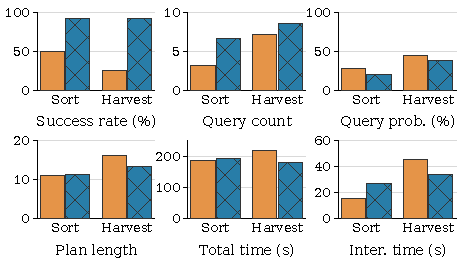
\includegraphics[width=\linewidth]{figures/05_PHYSICAL_BASELINE/exp_physical_vlm_group.pdf}
\caption{VLM responses}
\label{fig:physical_vlm}
\end{subfigure}%
\makebox[0.02\textwidth][c]{%
\raisebox{6pt}[0pt][0pt]{
\includegraphics[height=8pt]{figures/05_PHYSICAL_BASELINE/exp_physical_legend.pdf}}}%
\begin{subfigure}[b]{0.49\textwidth}
\centering
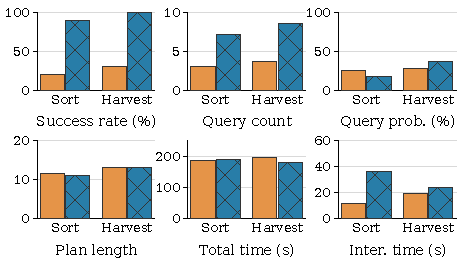
\includegraphics[width=\linewidth]{figures/05_PHYSICAL_BASELINE/exp_physical_human_group.pdf}
\caption{Human responses}
\label{fig:physical_human}
\end{subfigure}
\caption{Physical robot evaluation with VLM and human responses. (a) With VLM feedback, Ours achieves higher task success than KnowNo in both domains. (b) The same success advantage holds with human feedback.}
\label{fig:physical_results}
\end{figure*}



% \begin{table*}[t]
% \centering
% \caption{Physical robot results with VLM and human responses. Parentheses give successful trials over all trials. Other metrics report means over successful trials. A dash marks human results that are not yet available.}
% \label{tab:physical_robot_results}
% \small
% \setlength{\tabcolsep}{2.5pt}
% \begin{tabular*}{\textwidth}{@{\extracolsep{\fill}}lllccccccc}
% \toprule
% Source & Domain & Method & Success (\%) & \shortstack{Query\\count} & \shortstack{Query\\prob. (\%)} & \shortstack{Plan\\length} & \shortstack{Total\\time (s)} & \shortstack{Interaction\\time (s)} & \shortstack{Planning\\time (s)} \\
% \midrule
% VLM & Sort & KnowNo & 50.00 (20/40) & 3.15 & 28.64 & 11.00 & 186.51 & 15.46 & 20.08 \\
%  &  & Ours & 92.50 (37/40) & 6.70 & 19.81 & 11.24 & 193.69 & 26.83 & 1.11 \\
% \addlinespace
%  & Harvest & KnowNo & 25.00 (10/40) & 7.20 & 44.10 & 16.10 & 217.82 & 44.99 & 27.68 \\
%  &  & Ours & 92.50 (37/40) & 8.51 & 37.63 & 13.27 & 180.39 & 34.12 & 1.48 \\
% \midrule
% Human & Sort & KnowNo & 20.00 (2/10) & 2.90 & 26.09 & 11.50 & 184.48 & 11.59 & 16.94 \\
%  &  & Ours & 90.00 (9/10) & 7.20 & 18.18 & 11.00 & 190.15 & 36.49 & 0.94 \\
% \addlinespace
%  & Harvest & KnowNo & 30.00 (3/10) & 3.67 & 28.21 & 13.00 & 195.50 & 19.04 & 23.52 \\
%  &  & Ours & 10.00 (10/10) & 8.50 & 37.40 & 13.10 & 180.02 & 23.89 & 1.32 \\
% \bottomrule
% \end{tabular*}
% \end{table*}



Ours achieves $92.50\%$ success in both domains, compared with $50.00\%$ and $25.00\%$ for KnowNo in Sort and Harvest, respectively. Ours also requires less search time in both domains. Among successful Harvest trials, KnowNo uses $7.20$ queries compared with $8.51$ for Ours, yet executes longer plans and requires more total time, averaging $217.82$ seconds compared with $180.39$ seconds. In Sort, Ours achieves higher success but requires more time among successful trials. Mean total time is $193.69$ seconds for Ours and $186.51$ seconds for KnowNo. Mean interaction time is also longer at $26.83$ seconds compared with $15.46$ seconds. Ours therefore improves task success in both domains, while its advantage in total time is limited to Harvest. Query count alone does not explain total task time.
% Fewer queries therefore do not necessarily reduce execution costs.

We distinguish VLM response errors from planner failures. All three failures of Ours in each domain involve incorrect VLM feedback. In Sort, KnowNo has three VLM response failures and $17$ planner failures, with the latter involving autonomous action selections despite unmet preconditions. In Harvest, KnowNo has $18$ VLM response failures and $12$ planner failures. Six VLM failures involve repeated detection choices that exhaust the step limit despite feasible alternatives, and the remaining $12$ involve incorrect action selections.

These failures illustrate the importance of both query timing and query content. A single predicted action can still require state verification before execution. To select the correct action, the VLM must assess robot location, object states, and action preconditions. However, the VLM may still select an infeasible action or one that does not advance the task. Ours asks the VLM to verify current state facts and uses the updated belief for subsequent planning, leaving action selection to the planner.



% \begin{figure}[t]
% \centering
% 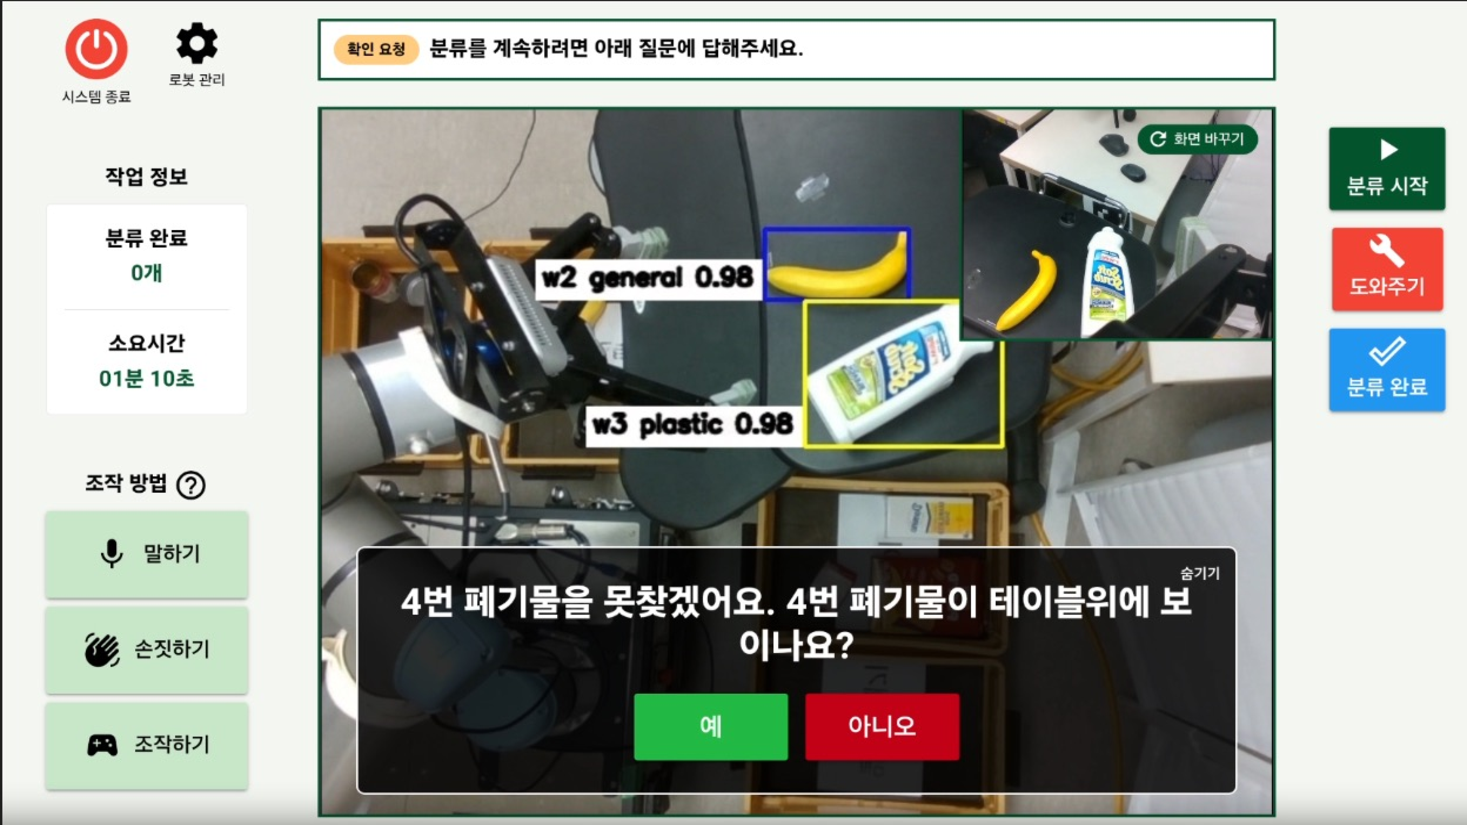
\includegraphics[width=\linewidth]{figures/exp_human_ui.pdf}
% \caption{Tablet interface used in the human evaluation. Participants view the robot camera feeds and select responses to robot queries.}
% \label{fig:human_tablet_interface}
% \end{figure}










\vspace{10pt}
\noindent\textbf{Human}\label{exp:human_eval}. 
We evaluate whether the oracle and VLM trends persist with human feedback using the same robot platforms and task domains. We recruited five participants (one man and four women), with a mean age of $26.4$ years (SD = $5.68$, range $18$--$33$). Each participant completes two trials per method and domain, yielding $10$ trials per condition. Participants receive task instructions and answer queries through the tablet interface. Domain and method orders vary across participants. Appendix~\ref{appx:user} provides the instructions and trial schedules. Fig.~\ref{fig:physical_results} reports the results.


Ours achieves $90.00\%$ success in Sort and $100.00\%$ in Harvest, compared with $20.00\%$ and $30.00\%$ for KnowNo, respectively, and requires less plan time in both domains. Across successful and failed trials, total interaction time divided by total query count gives $5.26$ seconds per query for Ours and $3.86$ for KnowNo in Sort, and $2.81$ and $6.42$ seconds in Harvest.


The higher Sort value for Ours is influenced by one P3 trial with $159.44$ seconds of interaction over nine queries. The experimenter observed hesitation after consecutive task failures. Excluding all eight P3 trials across both methods and domains gives $3.07$ seconds per query for Ours and $3.24$ for KnowNo in Sort, and $2.64$ and $4.99$ seconds in Harvest. This additional analysis shows that the relative interaction times in Sort are sensitive to prolonged responses from one participant.


The failure analysis identifies both incorrect human responses and autonomous planner decisions. In Sort, the single failure of Ours follows an incorrect confirmation that an object is visible. KnowNo has four human response failures involving placement before picking and four planner failures involving picking an undetected object without a query. In Harvest, Ours has no failures. Six KnowNo failures follow human selections that skip required preceding actions, and one follows incorrect perception of a rotten tomato without a state-verification query. These cases show that selecting the correct action requires participants to interpret execution prerequisites, while autonomous decisions can leave incorrect perception uncorrected.


% \begin{table}[!htbp]
% \centering
% \caption{Assigned order for the human evaluation. A denotes Ours and B denotes KnowNo. The method sequence applies to both domains for each participant.}
% \label{tab:human_assignment}
% \small
% \setlength{\tabcolsep}{3pt}
% \begin{tabular*}{\columnwidth}{@{\extracolsep{\fill}}cc@{}}
% \toprule
% Participant & Assigned order \\
% \midrule
% P1 & Sort $\rightarrow$ Harvest : $A\rightarrow A\rightarrow B\rightarrow B$ \\
% P2 & Harvest $\rightarrow$ Sort : $A\rightarrow B\rightarrow A\rightarrow B$ \\
% P3 & Sort $\rightarrow$ Harvest : $B\rightarrow B\rightarrow A\rightarrow A$ \\
% P4 & Harvest $\rightarrow$ Sort : $B\rightarrow A\rightarrow B\rightarrow A$ \\
% P5 & Sort $\rightarrow$ Harvest : $A\rightarrow A\rightarrow B\rightarrow B$ \\
% \bottomrule
% \end{tabular*}
% \end{table}



% Ours achieves a success rate of $90.00\%$ in Sort and $100.00\%$ in Harvest with human responses. KnowNo achieves $20.00\%$ and $30.00\%$ respectively. These results are consistent with the oracle and VLM comparisons and show that our method also achieves higher task success with human feedback. \cp{Ours also requires} less plan time than KnowNo. Mean plan time is $0.94$ seconds for Ours and $16.94$ seconds for KnowNo in Sort and $1.32$ and $23.52$ seconds in Harvest. Participants also need time to inspect the displayed information and choose a response. We compute the mean interaction time per query by dividing total interaction time by the total number of queries across successful and failed trials. The values are $5.26$ seconds for Ours and $3.86$ seconds for KnowNo in Sort and $2.81$ and $6.42$ seconds in Harvest.

% One Sort trial with Ours for P3 \cp{recorded} $159.44$ seconds of interaction over nine queries, including one query lasting $77.00$ seconds. The experimenter observed that P3 hesitated when answering after consecutive task failures in the preceding trials. To examine the influence of P3's interaction times, we repeat the calculation after excluding all eight of P3's trials, covering both Ours and KnowNo in both domains. The mean interaction time per query is then $3.07$ seconds for Ours and $3.24$ seconds for KnowNo in Sort and $2.64$ and $4.99$ seconds in Harvest.



% We also examine the failed trials with human responses. In Sort, the only failure of Ours occurs after a participant incorrectly confirms the presence of an object that is not visible. KnowNo fails in eight trials. In four trials, participants select a placement action before the robot has picked the object. In the other four, KnowNo selects a pick action without requesting assistance even though the object has not been detected. In Harvest, Ours completes all ten trials, whereas KnowNo fails in seven. Four failures occur after participants select scanning before the robot has picked the tomato. Two occur after participants select picking before detection at the new location, including one action entered as free text. The remaining failure occurs when KnowNo proceeds with harvesting a rotten tomato based on incorrect perception, without asking the participant to verify its condition. These cases show that answering an action-selection query requires participants to check which preceding actions have been completed. They also show that participants have no opportunity to correct an action if KnowNo proceeds without requesting assistance. 




% Plan times use the successful-trial values provided in the human experiment table.
% Ours achieves a success rate of $100.00\%$ in Sort and $50.00\%$ in Harvest with human responses. KnowNo achieves $16.67\%$ and $33.33\%$ respectively. Mean query counts are $6.00$ for Ours and $4.00$ for KnowNo in Sort and $9.67$ and $4.00$ in Harvest. Mean plan time is $1.09$ seconds for Ours and $20.40$ seconds for KnowNo in Sort and $1.46$ and $25.40$ seconds in Harvest. In Sort, interaction time and total time are $15.65$ and $167.45$ seconds for Ours compared with $10.78$ and $183.38$ seconds for KnowNo. In Harvest, the corresponding times are $27.00$ and $182.36$ seconds for Ours compared with $16.75$ and $181.89$ seconds for KnowNo. KnowNo uses $33.33\%$ fewer queries than Ours in Sort and $58.62\%$ fewer in Harvest. However the lower query counts do not consistently reduce total time. Plan lengths are similar across methods, with $11.00$ physical actions for both methods in Sort and $13.33$ for Ours and $13.00$ for KnowNo in Harvest. Despite the additional queries, Ours requires $8.69\%$ less total time in Sort and a similar total time in Harvest.

% \cp{Ours also achieves higher task success than KnowNo with human responses. These results suggest that query timing determines whether participants have an opportunity to correct robot decisions. Even if a participant notices an incorrect judgment, there may be no opportunity to correct it if the robot proceeds without a query. P1 reported that KnowNo proceeded without a query in situations where they wanted to intervene. Our method requests additional information if belief confidence is insufficient and incorporates human responses into subsequent planning.}





% \vspace{10pt}
% \noindent\textbf{Baseline Discussion}\label{exp:response_comparison}.
% Fig.~\ref{fig:response_comparison} shows that Ours achieves higher task success than KnowNo across oracle, VLM, and human feedback. The failure analyses suggest that both query timing and query content contribute to this difference. KnowNo failures include actions executed without a query despite incorrect perception or unmet preconditions, as well as actions selected by responders before the required preconditions are satisfied. These cases illustrate two requirements for effective queries. Query timing determines whether the responder can intervene before an incorrect action is executed. Query content determines the information and reasoning needed to provide a correct response.

% This distinction helps explain why query counts alone do not account for task success. In Harvest with VLM feedback, KnowNo asks $7.20$ questions on average compared with $8.51$ for Ours, yet their success rates are $25.00\%$ and $92.50\%$, respectively. Ours asks the responder to verify state facts and leaves action selection to the planner. This reduces the need for the responder to reason about action sequences, although incorrect state feedback can still cause failure. The baseline results support examining query timing and query content together. The following ablation experiments separate these components to assess their individual contributions.


% \begin{figure*}[!tp]
% \centering
% \begin{subfigure}[t]{0.495\textwidth}
% \centering
% 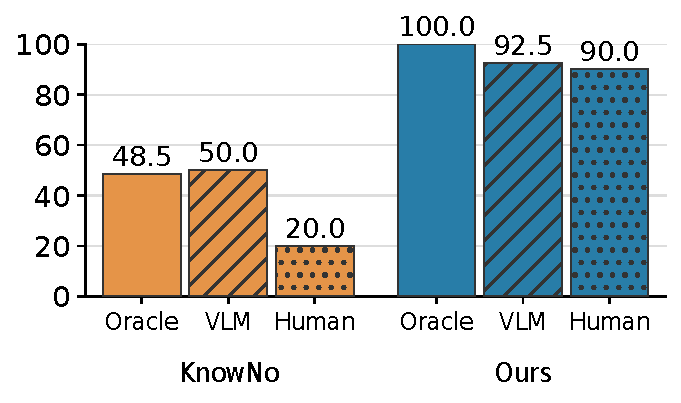
\includegraphics[width=\linewidth,height=.20\textheight,keepaspectratio]{figures/07_RESPONSE_COMPARISON/exp_response_waste_success.pdf}
% \caption{Sort Success rate (\%)}
% \label{fig:response_response_waste_success}
% \end{subfigure}
% \hfill
% \begin{subfigure}[t]{0.495\textwidth}
% \centering
% 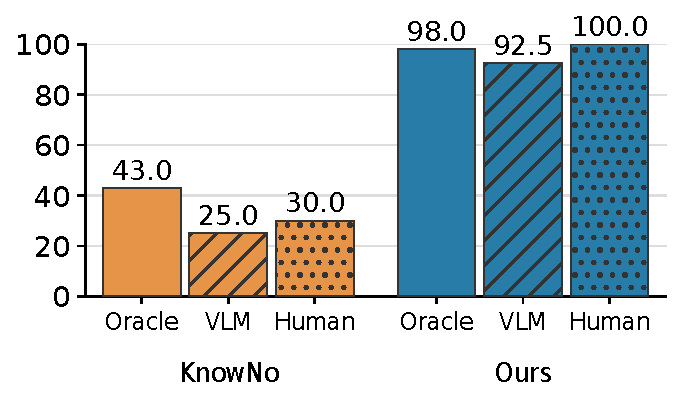
\includegraphics[width=\linewidth,height=.20\textheight,keepaspectratio]{figures/07_RESPONSE_COMPARISON/exp_response_tomato_success.pdf}
% \caption{Harvest Success rate (\%)}
% \label{fig:response_response_tomato_success}
% \end{subfigure}
% \par\medskip
% \begin{subfigure}[t]{0.495\textwidth}
% \centering
% 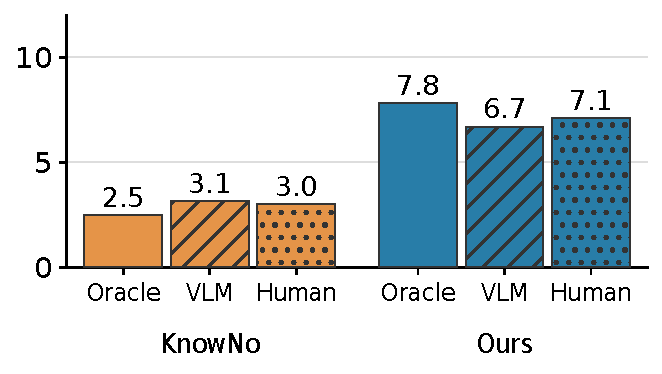
\includegraphics[width=\linewidth,height=.20\textheight,keepaspectratio]{figures/07_RESPONSE_COMPARISON/exp_response_waste_queries.pdf}
% \caption{Sort Query count}
% \label{fig:response_response_waste_queries}
% \end{subfigure}
% \hfill
% \begin{subfigure}[t]{0.495\textwidth}
% \centering
% 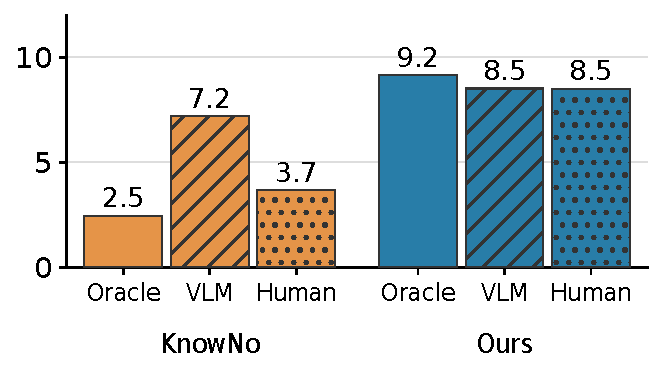
\includegraphics[width=\linewidth,height=.20\textheight,keepaspectratio]{figures/07_RESPONSE_COMPARISON/exp_response_tomato_queries.pdf}
% \caption{Harvest Query count}
% \label{fig:response_response_tomato_queries}
% \end{subfigure}
% \caption{Comparison across oracle, VLM, and human responses. Success rates are compared for Sort (a) and Harvest (b). Query counts are compared for Sort (c) and Harvest (d). Oracle trials use simulation, while VLM and human trials use physical robots.}\label{fig:response_comparison}
% \end{figure*}



% 

\subsubsection{Ablation Study}~\label{exp:when_what_random}\label{exp:policy_ablation}
% The ablation study isolates the effects of query timing and query selection on task success and query count. We compare seven configurations with oracle feedback.
The baseline comparison evaluates complete planning systems with different action planners and query policies. The ablation study examines the effects of query timing and query selection on task success and query count using seven configurations that share the POMCP action planner, with oracle feedback. For concise reference, we use \textbf{T} to label query timing variants and \textbf{S} to label query selection variants. With entropy gain selection fixed, we compare random (T1), conformal prediction (T2), and reward-based (T3) timing. With confidence timing fixed, we compare random (S1) and reward-based (S2) selection. R randomizes both query timing and query selection, while Ours combines confidence timing with entropy gain selection. Table~\ref{tab:query_strategy_matrix} summarizes these configurations. Each configuration has $200$ trials per domain. Table~\ref{tab:policy_ablation} and Fig.~\ref{fig:policy_ablation_results} present the results. Appendix~\ref{appx:ablation_configs} provides the query policy configurations.

\begin{figure}[!tp]
\centering
\captionsetup[subfigure]{font=footnotesize,skip=1pt}
\begin{minipage}[t]{0.5\columnwidth}
\vspace{0pt}
\begin{subfigure}[t]{\linewidth}
\centering
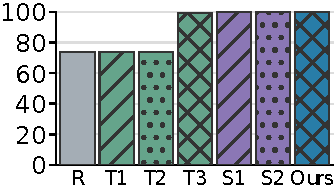
\includegraphics[width=\linewidth]{figures/08_ABLATION/exp_ablation_waste_success.pdf}
\caption{Sort Success rate (\%)}
\label{fig:ablation_ablation_waste_success}
\end{subfigure}
\par\vspace{1pt}
\begin{subfigure}[t]{\linewidth}
\centering
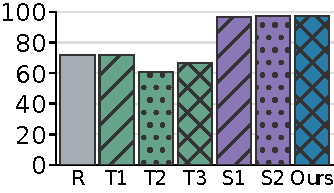
\includegraphics[width=\linewidth]{figures/08_ABLATION/exp_ablation_tomato_success.pdf}
\caption{Harvest Success rate (\%)}
\label{fig:ablation_ablation_tomato_success}
\end{subfigure}
\end{minipage}%
\begin{minipage}[t]{0.5\columnwidth}
\vspace{0pt}
\begin{subfigure}[t]{\linewidth}
\centering
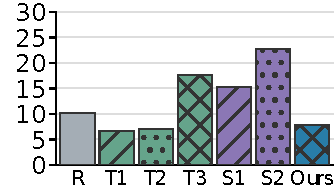
\includegraphics[width=\linewidth]{figures/08_ABLATION/exp_ablation_waste_queries.pdf}
\caption{Sort Query count}
\label{fig:ablation_ablation_waste_queries}
\end{subfigure}
\par\vspace{1pt}
\begin{subfigure}[t]{\linewidth}
\centering
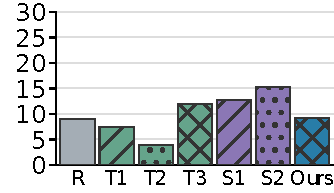
\includegraphics[width=\linewidth]{figures/08_ABLATION/exp_ablation_tomato_queries.pdf}
\caption{Harvest Query count}
\label{fig:ablation_ablation_tomato_queries}
\end{subfigure}
\end{minipage}
\caption{Results of the ablation study. (a)-(b) Confidence-based timing maintains high success rates in both domains. (c)-(d) Entropy-based selection reduces query counts compared with S1--S2. Our method achieves high task success while reducing query count.}
\label{fig:policy_ablation_results}
\end{figure}


\begin{table*}[t]
\centering
\caption{Query policy ablation. T1--T3 compare timing criteria and S1--S2 compare selection criteria. Highest success rates and lowest query counts are underlined, including ties.}
\label{tab:policy_ablation}
\label{tab:when_what_random}
\small
\setlength{\tabcolsep}{4pt}
\begin{tabular}{lllcccc}
\toprule
 & & & \multicolumn{2}{c}{Sort} & \multicolumn{2}{c}{Harvest} \\
\cmidrule(lr){4-5}\cmidrule(lr){6-7}
Condition & Timing & Selection & Success (\%) & Queries & Success (\%) & Queries \\
\midrule
R & Random & Random & 73.50 & $10.25 \pm 6.11$ & 72.00 & $9.08 \pm 3.94$ \\
T1 & Random & Entropy Gain & 73.50 & $\underline{6.65} \pm 3.29$ & 72.00 & $7.44 \pm 2.73$ \\
T2 & Conformal Prediction & Entropy Gain & 74.00 & $7.09 \pm 2.58$ & 60.50 & $\underline{3.91} \pm 1.71$ \\
T3 & Reward & Entropy Gain & 99.00 & $17.65 \pm 2.89$ & 66.50 & $12.02 \pm 2.88$ \\
S1 & Confidence & Random & \underline{100.00} & $15.21 \pm 3.53$ & 96.50 & $12.70 \pm 2.53$ \\
S2 & Confidence & Reward & \underline{100.00} & $22.79 \pm 6.26$ & 97.00 & $15.27 \pm 2.95$ \\
\textbf{Ours} & Confidence & Entropy Gain & \textbf{\underline{100.00}} & $\boldsymbol{7.83 \pm 2.16}$ & \textbf{\underline{97.50}} & $\boldsymbol{9.16 \pm 1.91}$ \\
\bottomrule
\end{tabular}
\end{table*}

The timing comparison evaluates R, T1--T3, and Ours. In Sort, R and T1 achieve $73.50\%$ success, and T2 achieves $74.00\%$. T3 achieves $99.00\%$ compared with $100.00\%$ for Ours, but requires $17.65$ queries compared with $7.83$. R, T1, and T2 use $10.25$, $6.65$, and $7.09$ queries respectively. In Harvest, R and T1 achieve $72.00\%$ success, while T2 and T3 achieve $60.50\%$ and $66.50\%$ compared with $97.50\%$ for Ours. Mean query counts are $9.08$ for R, $7.44$ for T1, $3.91$ for T2, $12.02$ for T3, and $9.16$ for Ours.

These results show that task success depends on the query trigger as well as query selection. T1 replaces random selection in R with entropy gain and reduces query count without improving success. Random timing can miss necessary verification because the trigger does not depend on current state uncertainty. T2 can also end queries after the action prediction set narrows to one candidate, even if the state facts required to execute the candidate action remain uncertain. T3 uses expected task reward to determine whether to initiate queries, then selects queries by entropy gain and repeats verification until confidence reaches $\tau$. In Sort, object category verification directly informs the correct bin choice and task reward, so repeated verification may support the high success rate of $99.00\%$. However T3 requires $125.42\%$ more queries than Ours. In Harvest, T3 uses $31.22\%$ more queries than Ours, but the success rate of T3 is $31.00$ percentage points lower. Therefore reward-based timing can request more queries overall and still fail to verify necessary state information at the appropriate time. Thus Ours uses current state confidence as the query trigger and achieves the highest success in both domains with fewer queries than reward-based timing.

With confidence-based query timing fixed, different query selection strategies maintain high success rates but require different numbers of queries. The query selection comparison evaluates R, S1, S2, and Ours. R achieves $73.50\%$ success in Sort and $72.00\%$ in Harvest with $10.25$ queries in Sort and $9.08$ in Harvest. S1 retains random selection but uses confidence timing, and success increases to $100.00\%$ and $96.50\%$ respectively. With confidence timing fixed, S1, S2, and Ours all achieve $100.00\%$ success in Sort. Mean query counts are $15.21$ for S1, $22.79$ for S2, and $7.83$ for Ours. In Harvest, S1 and S2 achieve $96.50\%$ and $97.00\%$ success, respectively, compared with $97.50\%$ for Ours. Mean query counts are $12.70$ for S1, $15.27$ for S2, and $9.16$ for Ours.

Confidence timing maintains $100.00\%$ success in Sort and at least $96.50\%$ in Harvest across all three query selection strategies. Under confidence timing, query selection primarily affects the number of queries needed to reach the required confidence. Random selection does not prioritize facts by their expected reduction in state uncertainty. Reward-based selection evaluates expected task reward without directly measuring the information provided by a query response. Entropy gain selects facts according to the expected reduction in state uncertainty, so the selection criterion matches the confidence requirement that ends a query episode. Relative to S1 and S2, Ours reduces query count by $48.52\%$ and $65.64\%$ in Sort and by $27.87\%$ and $40.01\%$ in Harvest. Thus our query selection method reduces the number of queries required under confidence timing without reducing task success.

These results support the main contribution of our method through the distinct roles of query timing and query selection. Query timing determines whether the robot requests additional information before it executes actions under state uncertainty. Confidence timing achieves high success with random, reward-based, and entropy gain selection, while entropy gain under random timing reduces query count without improving success over R. Once confidence timing establishes a high success level, entropy gain reduces the number of queries needed to reach the required confidence. Therefore our method combines a timing criterion that supports task success with a selection criterion that reduces query count at that success level.

\subsubsection{Threshold Experiments}~\label{exp:sys_threshold}
After the ablation comparison, we examine how the confidence threshold controls task success and query count. We vary $\tau$ from $0.0$ to $1.0$ in increments of $0.1$ with entropy gain selection fixed and correct oracle responses in simulation. Each threshold has $200$ trials per domain. At $\tau=0.8$, we reuse the Ours trials reported in Tables~\ref{tab:baseline_results} and~\ref{tab:policy_ablation}. Fig.~\ref{fig:threshold_results} presents the results.

\begin{figure}[!tp]
\centering
\begin{subfigure}[t]{0.5\columnwidth}
\centering
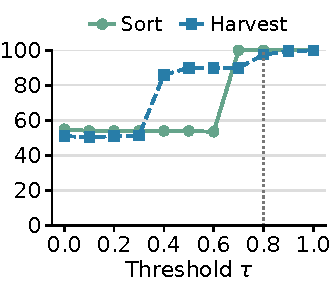
\includegraphics[width=\linewidth]{figures/09_THRESHOLD/exp_threshold_success.pdf}
\caption{Task success}
\label{fig:threshold_success}
\end{subfigure}%
\begin{subfigure}[t]{0.5\columnwidth}
\centering
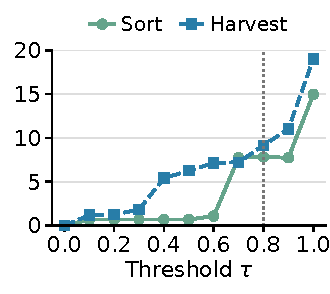
\includegraphics[width=\linewidth]{figures/09_THRESHOLD/exp_threshold_queries.pdf}
\caption{Mean query count}
\label{fig:threshold_queries}
\end{subfigure}
\caption{Effect of the confidence threshold $\tau$ on task success and query count. (a) Task success reaches $100.00\%$ at $\tau=0.7$ in Sort and $100.00\%$ at $\tau=1.0$ in Harvest. (b) Mean query count increases sharply at $\tau=1.0$ in both domains. Relative to the default $\tau=0.8$ (dotted line), $\tau=1.0$ roughly doubles query count while success remains unchanged in Sort and increases by $2.50\%p$ in Harvest.}
\label{fig:threshold_results}
\end{figure}

Fig.~\ref{fig:threshold_results} shows different responses to the confidence threshold across the two domains. In Sort, success increases from $53.50\%$ at $\tau=0.6$ to $100.00\%$ at $\tau=0.7$ and remains unchanged at higher thresholds. Mean query counts range from $7.74$ to $7.83$ over $\tau=0.7$--$0.9$ and increase to $14.97$ at $\tau=1.0$. In Harvest, success rises from $51.50\%$ at $\tau=0.3$ to $86.00\%$ at $\tau=0.4$ and remains $90.00\%$ over $\tau=0.5$--$0.7$. Further increases in the threshold yield $97.50\%$ success at $\tau=0.8$, $99.50\%$ at $\tau=0.9$, and $100.00\%$ at $\tau=1.0$. Mean query count increases from $5.41$ at $\tau=0.4$ to $9.16$ at $\tau=0.8$ and $19.00$ at $\tau=1.0$.

System-initiated querying improves task success under the same POMCP action planner. Without queries ($\tau=0.0$), Ours achieves $55.00\%$ success in Sort and $51.00\%$ in Harvest. Both rates exceed those of KnowNo and IntroPlan with oracle feedback. At $\tau=0.8$, success increases by $45.00$ and $46.50$ percentage points, respectively. Successful trials require an average of $7.83$ queries in Sort and $9.16$ in Harvest.

Additional queries provide limited gains once task success approaches its maximum. Raising $\tau$ from $0.8$ to $1.0$ increases mean query count by $91.19\%$ in Sort and $107.42\%$ in Harvest, but success increases by $0.00$ and $2.50$ percentage points, respectively. In Harvest, the final increase from $\tau=0.9$ to $1.0$ alone adds $7.98$ queries for only $0.50$ percentage points of additional success. We use $\tau=0.8$ as a common threshold to balance task success and query count across both domains.


\subsubsection{Interviews}\label{exp:interviews}
% We interview all five participants after they experience both methods in Sort and Harvest. Participants describe Ours as asking them to verify the current state and KnowNo as asking them to choose the next action. In KnowNo, P1 expects some action choices to include preceding steps, P2 is unsure whether all candidate actions are currently executable, and P4 considers which steps have to occur first. These reports suggest that answering action-selection queries requires participants to interpret both what each action executes and which preconditions have to be satisfied. Differences in these interpretations help explain the action-selection failures analyzed earlier.
We interview all five participants after they use Ours and KnowNo in both domains. P1 and P2 describe Ours as more reliable than KnowNo for completing the evaluated tasks. P1 considers errors less likely with Ours. P2 expects Ours to complete the task after receiving state confirmations, whereas KnowNo sometimes fails after P2 selects actions that appear executable from the camera view.

% Four participants (P1--P4) prefer Ours for the evaluated tasks. P1 and P2 describe smoother task progress and greater perceived efficiency, while P3 and P4 emphasize convenience and less deliberation about subsequent actions. P3 finds frequent questions bothersome despite preferring Ours, and P5 prefers KnowNo because directly selecting or entering a command feels more convenient than repeated confirmations. Interview results indicate that preferences reflect both the judgments required to answer queries and the frequency and form of participation.
Selecting the correct action requires participants to interpret both the scope of each action and the preceding steps needed for execution. P1 expects KnowNo to perform picking as part of a subsequent action, such as checking tomato quality. P3 recalls a failure after selecting a quality check before picking, and P4 attributes a tomato-task failure to skipping a required stage. The reported failures match the failure analysis, which identifies KnowNo failures following selections that omit required preceding actions. Ours asks participants to verify state facts and leaves action selection and sequencing to the planner. Participants therefore do not need to determine whether an action choice includes the necessary preceding steps. This division of responsibilities helps explain the higher task success rate of Ours in the human evaluation.


\subsubsection{Discussion and Limitation}\label{exp:discussion}
We find that query timing primarily affects task success, while query selection primarily affects the number of queries required. The ablation study shows that confidence-based timing maintains high success across selection strategies, while entropy-based selection reduces query counts when timing is fixed. Our method combines confidence-based timing with entropy-based selection to balance task success and query efficiency. Across Sort and Harvest, our method achieves the highest task success among the evaluated methods in simulation and with VLM and human feedback on physical robots.



Efficient query selection reduces the number of queries needed to reach a given confidence level. The confidence threshold controls the trade-off between accepting uncertainty and requesting further verification. If $\tau<1$, the robot may commit to a state while alternative states retain belief weight. Accepting uncertainty can reduce query counts, but an incorrect state estimate may affect subsequent actions. If $\tau=1$, the robot resumes execution only after belief entropy reaches zero. Our threshold experiments show that increasing the number of queries does not necessarily improve task success rates. The benefit of additional queries depends on whether the remaining uncertainty affects task success. The two domains also require different confidence levels to achieve a high task success rate. 



A limitation of our method is that the belief update does not account for errors in responses from external agents. State hypotheses inconsistent with answers are removed regardless of response reliability. Incorrect feedback can therefore exclude the true state from the belief and leave the robot confident in an incorrect state. The failures involving incorrect VLM and human responses illustrate the practical impact of feedback errors. Raising the confidence threshold cannot ensure a correct state estimate, because confidence is computed over the remaining hypotheses. Incorporating response reliability into the belief update could preserve plausible alternatives by adjusting hypothesis weights instead of removing inconsistent hypotheses outright.

% % Keep the experimental figures and tables before the conclusion.
% \clearpage
